\documentclass[xcolor=pdftex,dvipsnames,table,aspectratio=169]{beamer}
%\documentclass[xcolor=pdftex,dvipsnames,table,handout,aspectratio=169]{beamer}

%\setbeameroption{show notes}

\usepackage{bm,graphicx,multirow,amsmath,tikz} %fancybox,
\usepackage{color}%,textpos}
\usepackage[round]{natbib}
\usepackage[normalem]{ulem}
\usepackage{hyperref}
\usepackage{lastpage}
\usepackage{array}
\usepackage{color}
\usepackage{framed}
\usepackage{hyperref}

% Define Western colours
\definecolor{western}{rgb}{.306,.152,.524}
\definecolor{westerngray}{rgb}{.512,.508,.524}

%% Define BEAMER colours
\setbeamercolor{frametitle}{bg=western,fg=white}
\setbeamercolor{framesubtitle}{bg=western,fg=black}
\setbeamercolor{title}{fg=white,bg=western}
\setbeamercolor{author}{fg=white,bg=western}
\setbeamercolor{institute}{fg=white,bg=western}
\setbeamercolor{date}{fg=white,bg=western}

%% Set BEAMER fonts
\setbeamerfont{title}{shape=\bf}
\setbeamerfont{frametitle}{shape=\sc,size=\Large}
\setbeamerfont{framesubtitle}{shape=\sc,size=\Large}
\setbeamerfont{footline}{shape=\sc}

%% Define BEAMER toc
\setbeamercolor{section in toc}{fg=western}
\setbeamercolor{subsection in toc}{fg=westerngray}
\setbeamertemplate{sections/subsections in toc}[ball]

%% Define BEAMER background
\setbeamercolor{background canvas}{bg=white}

%% Define BEAMER footer
\setbeamertemplate{navigation symbols}{}
\setbeamercolor{footline}{fg=white,bg=western}
\setbeamertemplate{footline}{%
  \begin{beamercolorbox}[wd=\paperwidth]{footline}
    \vskip5pt

    \raisebox{.05in}{
      \scriptsize{\bf \insertshorttitle}
    }
    \hfill
    \raisebox{.05in}{
      \scriptsize{\bf \insertframenumber/\inserttotalframenumber} 
    }
    \hspace{5pt}

    \vskip5pt
  \end{beamercolorbox}
}

%% Define BLOCK environment
\setbeamercolor{block title}{fg=western}
\setbeamerfont{block title}{series=\bfseries}

%% Define ENUMERATE and ITEMIZE environements
\setbeamertemplate{itemize item}[ball]
\setbeamertemplate{enumerate item}[ball]
\setbeamercolor{item projected}{bg=western}

%% Define BEAMER toc
\setbeamercolor{sections/subsections in toc}{fg=blue!75}
\setbeamertemplate{sections/subsections in toc}[ball]

% %% Define SECTION openings
% \AtBeginSection[]{
%   \begin{frame}{\insertshorttitle}
%     \tableofcontents[currentsection,subsectionstyle=hide/hide/hide]
    
%   \end{frame}
% }

%% Define BEAMER frametitle
\addtobeamertemplate{frametitle}{
   \let\insertframetitle\insertsectionhead}{}
\addtobeamertemplate{frametitle}{
   \let\insertframesubtitle\insertsubsectionhead}{}


\makeatletter
  \CheckCommand*\beamer@checkframetitle{\@ifnextchar\bgroup\beamer@inlineframetitle{}}
  \renewcommand*\beamer@checkframetitle{\global\let\beamer@frametitle\relax\@ifnextchar\bgroup\beamer@inlineframetitle{}}
\makeatother

% Define counters for example and exercise
\newcounter{example}
\newcounter{exercise}

% Define example and exercise commands
\renewcommand{\example}
{\stepcounter{example}Example \lecturenum.\arabic{example}}
\newcommand{\examplectd}
{Example \lecturenum.\arabic{example}\ ctd}
\newcommand{\exercise}
{\stepcounter{exercise}Exercise \lecturenum.\arabic{exercise}}
\newcommand{\exercisectd}
{Exercise \lecturenum.\arabic{exercise}\ ctd}

\usepackage{enumitem}

\newcommand{\lecturenum}{16}

\title[SS2857]{Probability and Statistics I}
\subtitle{16. The Normal Distribution}

\date{}

%% Add logo
% \titlegraphic{\includegraphics[height=2cm]{../uwo_logo_reversed}}

%% Initialize R


\begin{document}

{
\setbeamertemplate{footline}{}
\setbeamercolor{background canvas}{bg=western}

\begin{frame}
  \addtocounter{framenumber}{-1}

  \maketitle
\end{frame}
}

\section{Review}

\begin{frame}<handout:0>
  Suppose that $X$ is a continuous random variable with pdf $f(x)$ and cdf $F(x)$.
  \begin{enumerate}[label=\alph*),start=1]
  \item TRUE or FALSE: $f(x) \leq 1$ for all $x \in \mathbb R$
  \item TRUE or FALSE: $f(x)$ is continuous
  \item TRUE or FALSE: $E(X^2) \geq E(X)^2$
  \item Which of the following is not equal to all of the others?
    \begin{tabular}{cc}
      A) $P(3 \leq X \leq 5)$ & B) $P(3 < X \leq 5)$\\
      C) $P(3 < X < 5)$ & D) $P(3 < X < 4) + P(4 < X < 5)$
    \end{tabular}
  \end{enumerate}
\end{frame}

\section{The Normal Distribution}

\begin{frame}
  \frametitle{\invisible{Hello}}
  
  \begin{center}
    \Large{\textbf{4.3 The Normal Distribution}}
  \end{center}
  
  \bigskip
  
  % \only<1>{
  %   \begin{center}
  %     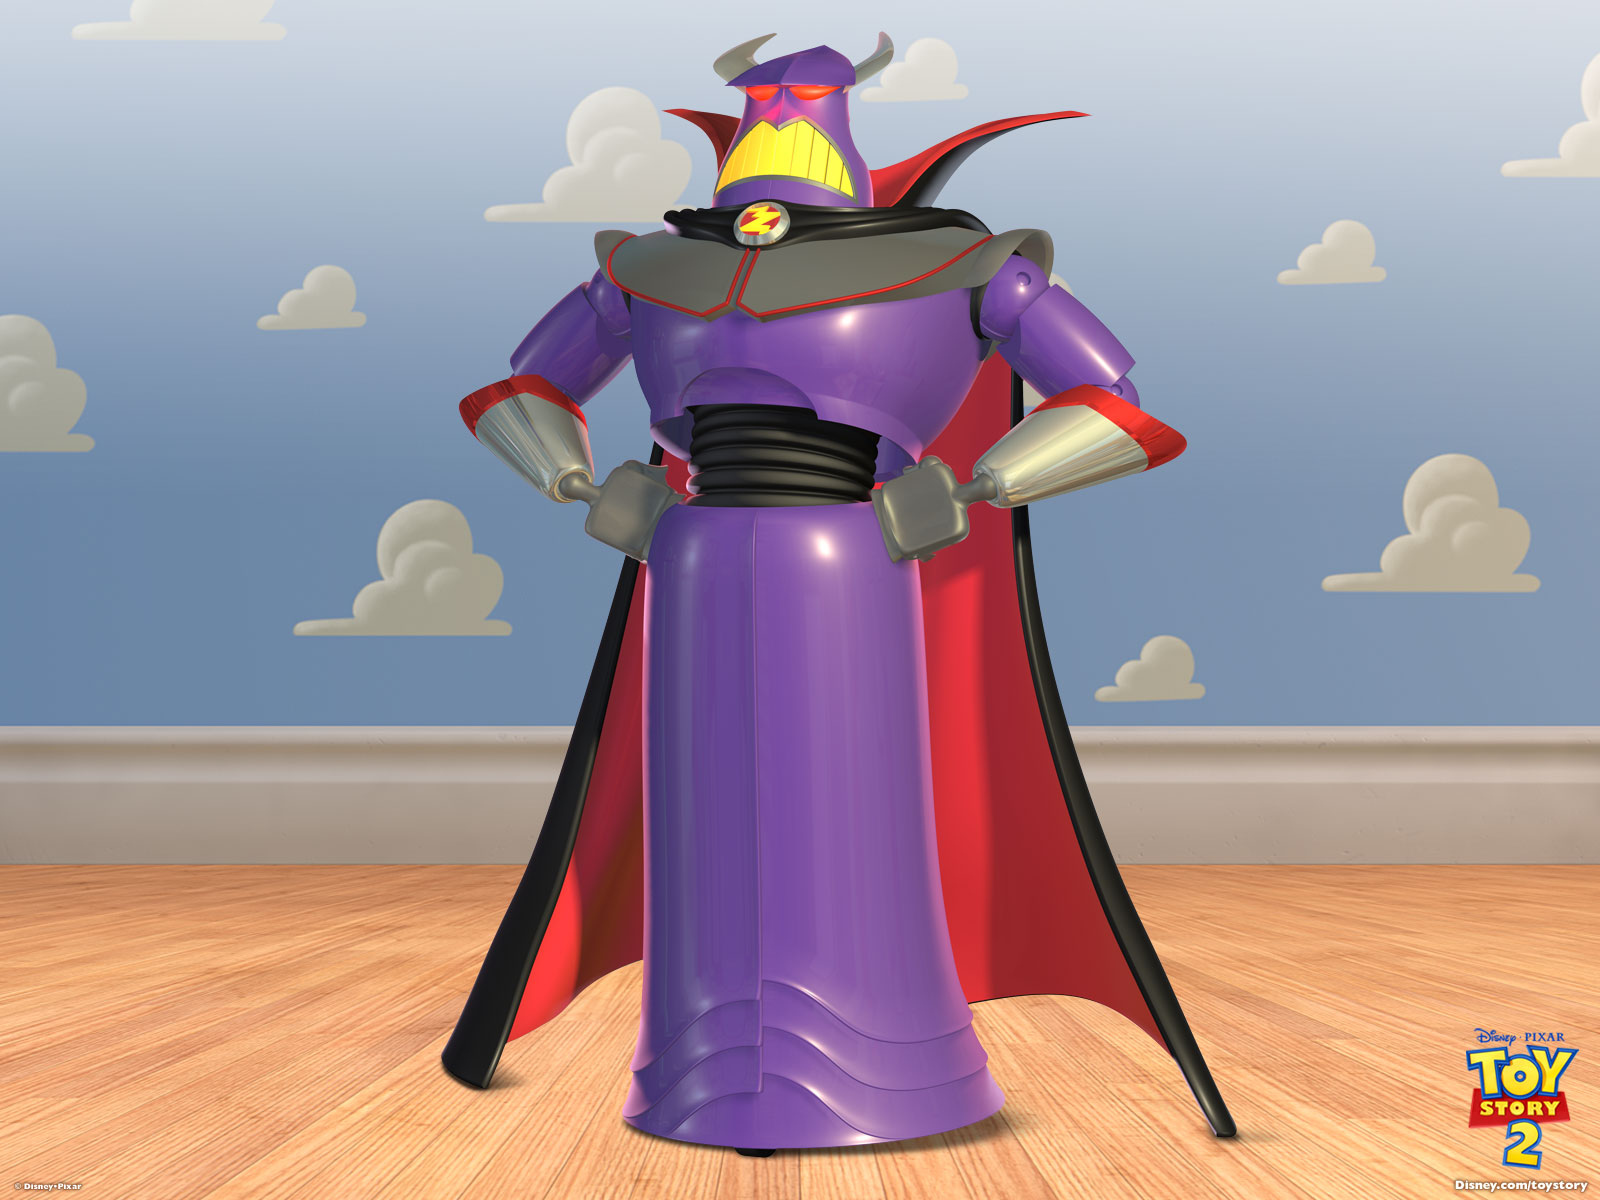
\includegraphics[height=.5\textheight]{zurg}
  %   \end{center}
  % }
\end{frame}

\begin{frame}
  
  \begin{block}{The Normal Distribution}
    We say that a random variable $X$ has a normal distribution with mean $\mu$ and variance $\sigma^2$ if the pdf of $X$ is
    \[
      f(x;\mu,\sigma)=\frac{1}{\sqrt{2\pi}\sigma} \exp\left(-\frac{(x-\mu)^2}{2\sigma^2}\right)
    \]
    for all $x \in \Re$. 
    
    \bigskip
    
    Mathematically, we write $ X \sim \mbox{Normal}(\mu,\sigma^2)$.
  \end{block}
\end{frame}

\begin{frame}
  \begin{block}{Properties}
%    \begin{columns}
%      \begin{column}{.5\textwidth}
        \begin{itemize}
        \item CDF: No closed form

       %\item MGF: $M_X(t)=e^{\mu t + \sigma^2t^2/2}$

        \item Mean: $E(Z)=\mu$
%        \end{itemize}
%      \end{column}
      
%      \begin{column}{.5\textwidth}
%        \begin{itemize}
        \item Variance: $V(Z)=\sigma^2$

%        \item Skewness: $0$
        \end{itemize}
%      \end{column}
%    \end{columns}
  \end{block}
  
  \begin{block}{Calculator}
  \url{https://stattrek.com/online-calculator/normal}
  \end{block}
\end{frame}

\begin{frame}
  \begin{block}{\example}
    The adult heights of people assigned to be male and female at birth can be modelled amazingly well by a normal distribution. Suppose that the adult height people assigned to be female at birth is normally distributed with mean 64 inches and standard deviation 3 inches.
    \[
      X \sim \mbox{Normal}(64,9).
    \]
    
    \begin{enumerate}[label=\alph*),start=1]
    \item What is the density of $X$?
    \item What is the probability that someone assigned to be female at birth will be:
      \begin{enumerate}[label=\roman*),start=1]
      \item less than 5 feet tall? 
      \item greater than 6 feet tall?
      \item between 5 and 6 feet tall?
      \end{enumerate}
    \item Find values $l$ and $u$ such that $P(l < X < u) \approx .95$. 
    \end{enumerate}
  \end{block}
\end{frame}




\begin{frame}

  \begin{block}{\examplectd}
  \begin{center}
    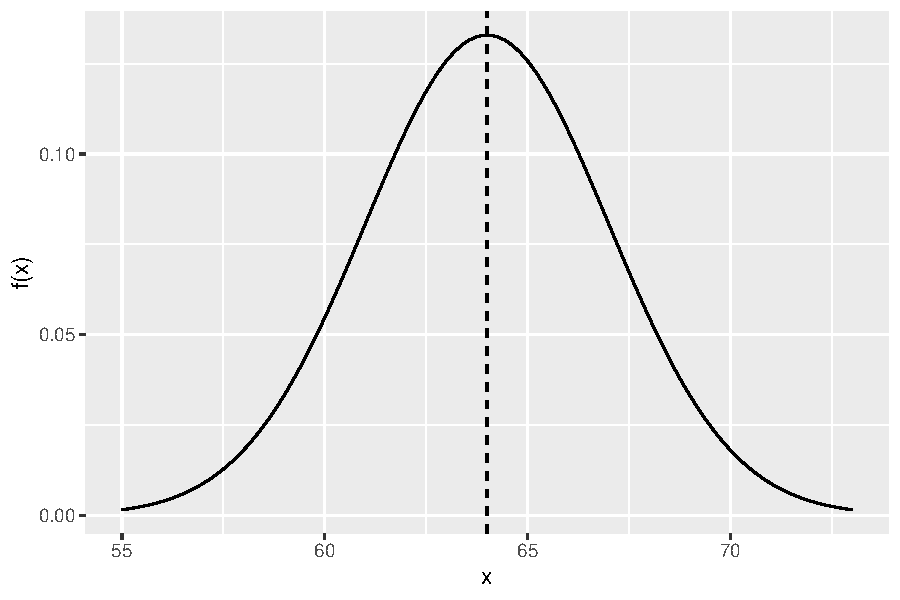
\includegraphics[height = .8\textheight]{figure/exercise-20-1}
  \end{center}
  \end{block}
  
\end{frame}

\begin{frame}<handout:0>
  \begin{block}{\examplectd}
    The adult heights of people assigned to be male and female at birth can be modelled amazingly well by a normal distribution. Suppose that the adult height people assigned to be female at birth is normally distributed with mean 64 inches and standard deviation 3 inches:
    \[
      X \sim \mbox{Normal}(64,9).
    \]
    
    \begin{enumerate}[label=\alph*),start=1]
    \item What is the density of $X$?
    \item What is the probability that someone assigned to be female at birth will be:
      \begin{enumerate}[label=\roman*),start=1]
      \item less than 5 feet tall? 
      \item greater than 6 feet tall?
      \item between 5 and 6 feet tall?
      \end{enumerate}
    \item Find values $l$ and $u$ such that $P(l < X < u) \approx .95$. 
    \end{enumerate}
  \end{block}
\end{frame}

\begin{frame}

  \begin{block}{\examplectd}
    \begin{center}
    \begin{tabular}{ccc}
    $P(X < 60)$ & $P(X > 72)$ & $P(60 < X < 72)$
    \\
    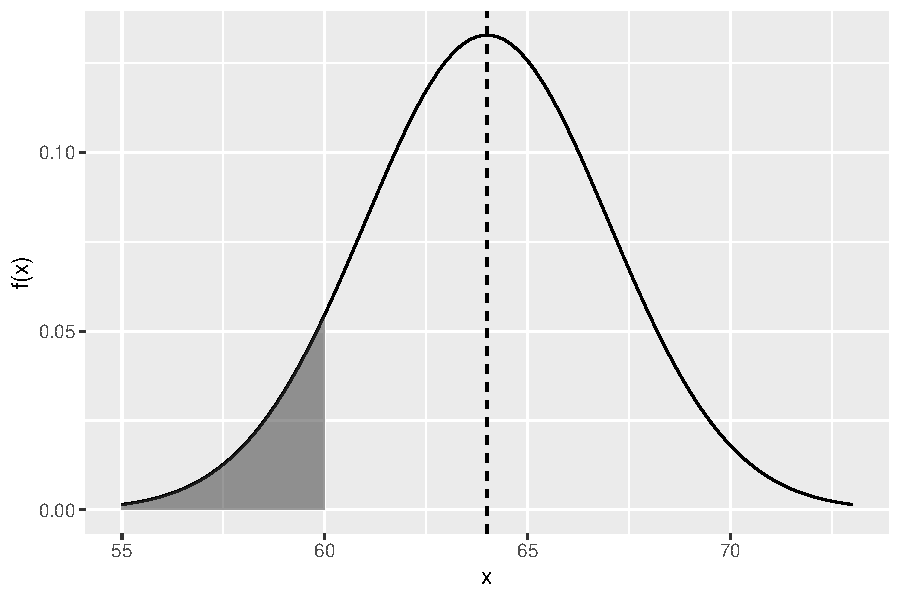
\includegraphics[height = .35\textheight]{figure/exercise-20-2}
      &
        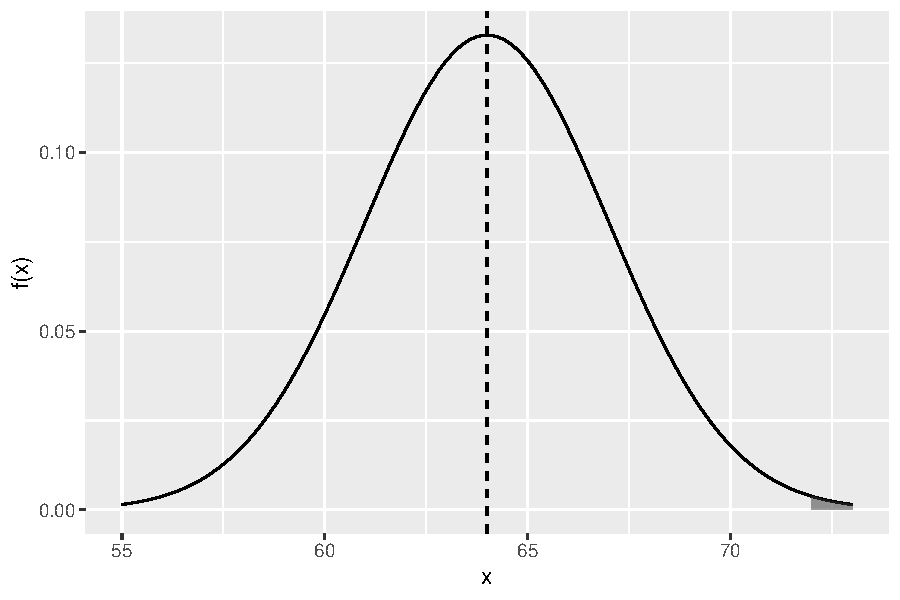
\includegraphics[height = .35\textheight]{figure/exercise-20-3}
        &
      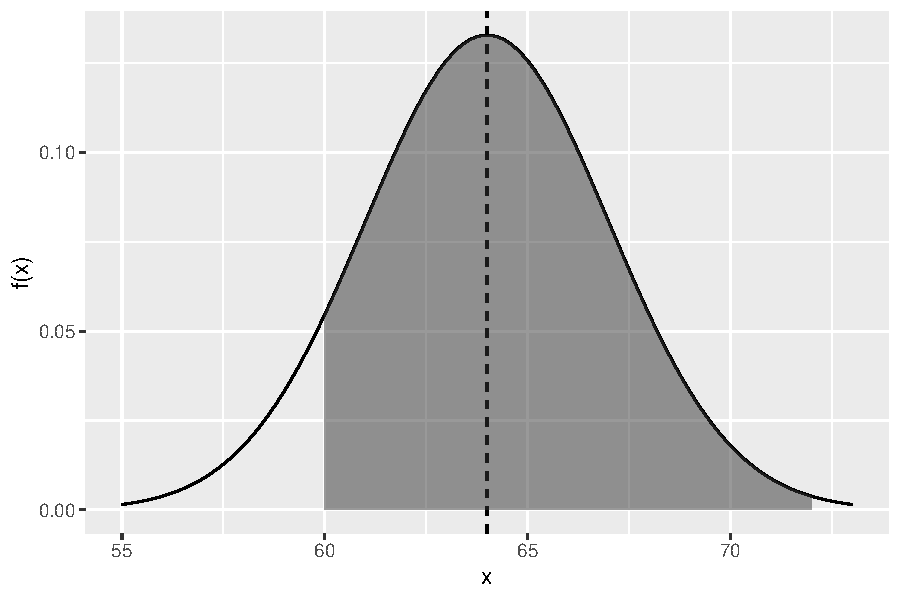
\includegraphics[height = .35\textheight]{figure/exercise-20-4}
    \end{tabular}
    \end{center}
  \end{block}
  
\end{frame}

\begin{frame}
  
  \begin{block}{The Standard Normal Distribution}
    We say that a random variable $Z$ has a \textbf{standard} normal distribution if 
    $$
    Z \sim \mbox{Normal}(0,1).
    $$
    The pdf of the standard normal is
    \[
      f(x)=\frac{1}{\sqrt{2\pi}} \exp\left(-\frac{z^2}{2}\right)
    \]
    for all $x \in \Re$. 
  \end{block}
\end{frame}

\begin{frame}
  \begin{block}{Properties}
        \begin{itemize}
        \item CDF: No closed form

        \item Mean: $E(Z)=0$
        \item Variance: $V(Z)=1$
        \end{itemize}
  \end{block}
\end{frame}

\begin{frame}

  \begin{block}{\examplectd}
    \begin{center}
    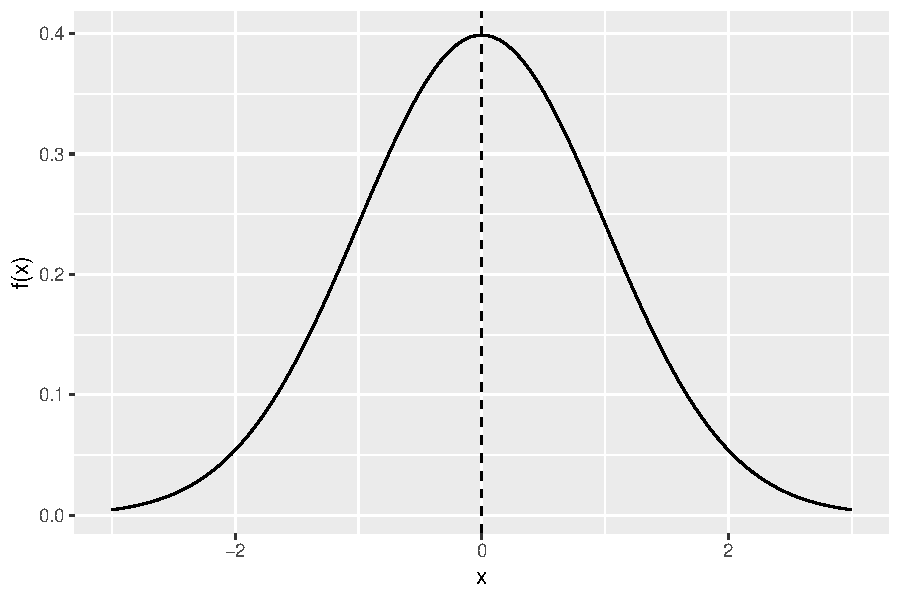
\includegraphics[height = .8\textheight]{figure/exercise-20-5}
    \end{center}
  \end{block}
  
\end{frame}

\begin{frame}
  \begin{block}{Standardization}
    If $X \sim \mbox{Normal}(\mu,\sigma^2)$ then
    \[
      Z=\frac{X-\mu}{\sigma}
    \]
    has a standard normal distribution.

    \bigskip

    \pause
    
    We can use this fact to compute probabilities for any normal random variable from the probabilities of a standard normal random variable:
    \[
      P(X \leq x)
      =P\left(\frac{X-\mu}{\sigma} \leq \frac{x-\mu}{\sigma}\right)
      =P\left(Z \leq \frac{x-\mu}{\sigma}\right)
    \]
    where $Z \sim \mbox{Normal}(0,1)$. 
  \end{block}
\end{frame}

\begin{frame}<handout:0>
  \begin{block}{\examplectd}
    The adult heights of people assigned to be male and female at birth can be modelled amazingly well by a normal distribution. Suppose that the adult height people assigned to be female at birth is normally distributed with mean 64 inches and standard deviation 3 inches:
    \[
      X \sim \mbox{Normal}(64,9).
    \]
    
    \begin{enumerate}[label=\alph*),start=4]
    \item Repeat part b) using standardization
    \end{enumerate}
  \end{block}
\end{frame}

\begin{frame}

  \begin{block}{\examplectd}
    \begin{center}
    \begin{tabular}{ccc}
    $P(X < 60)$ & $P(X > 72)$ & $P(60 < X < 72)$
    \\
    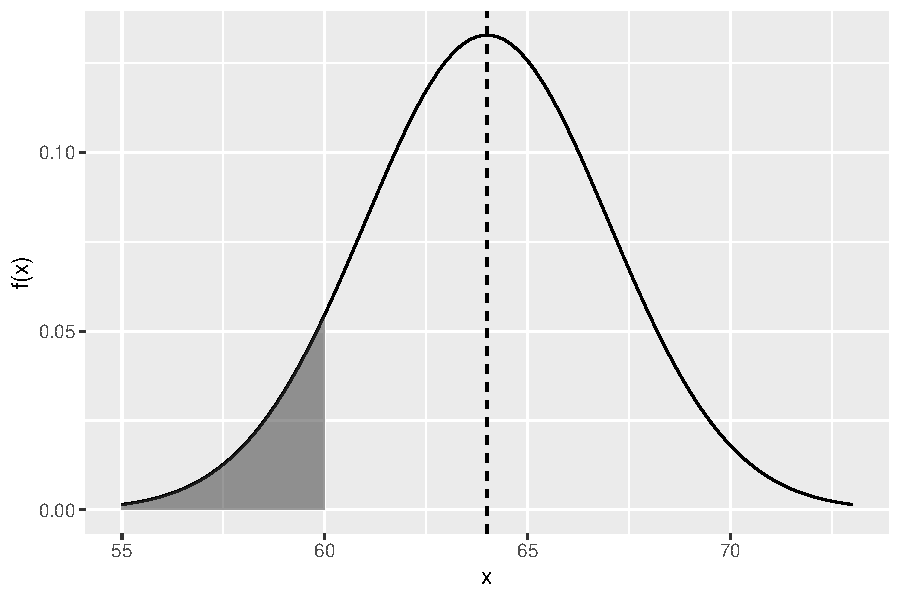
\includegraphics[height = .35\textheight]{figure/exercise-20-2}
      &
        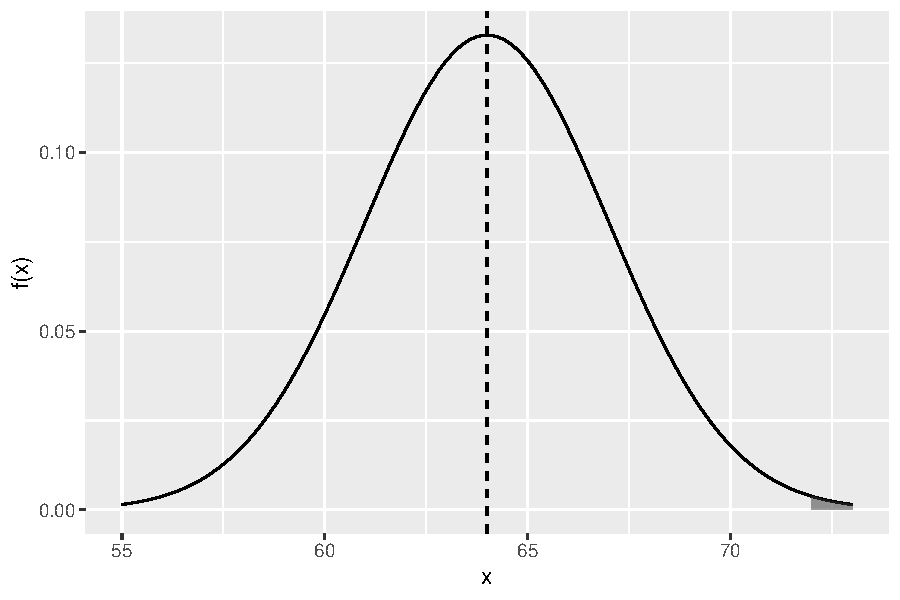
\includegraphics[height = .35\textheight]{figure/exercise-20-3}
        &
      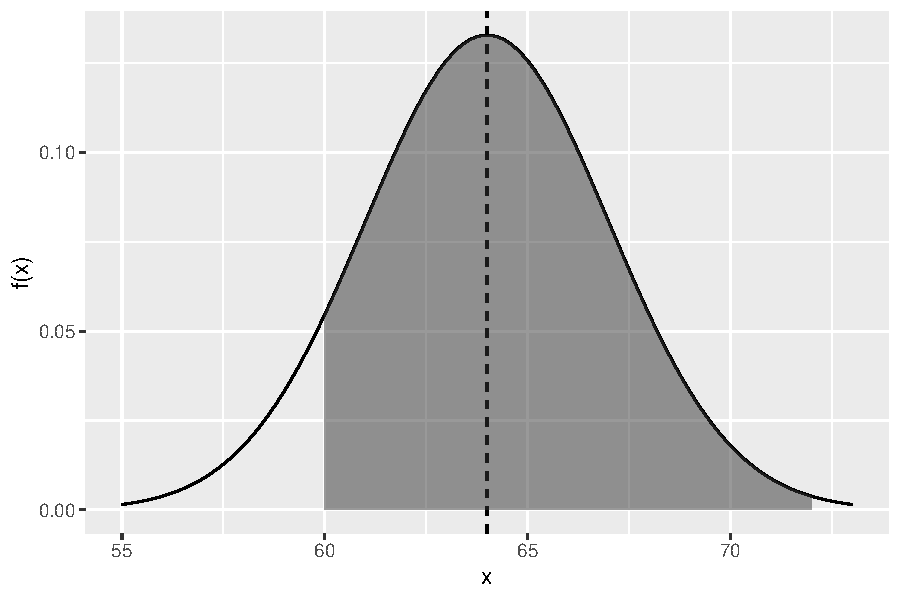
\includegraphics[height = .35\textheight]{figure/exercise-20-4}
    \end{tabular}
    \end{center}
  \end{block}
  
\end{frame}

\begin{frame}

  \begin{block}{\examplectd}
    \begin{center}
    \begin{tabular}{ccc}
    $P\left(Z < \frac{(60-64)}{3}\right)$
    & $P\left(Z > \frac{(72-64)}{3}\right)$
    & $P\left(\frac{(60-64)}{3} < Z < \frac{(72-64)}{3}\right)$\\
    $=P(Z < -4/3)$ & 
    $=P(Z > 8/3)$ &
    $=P(-4/3 < Z < 8/3)$\\
    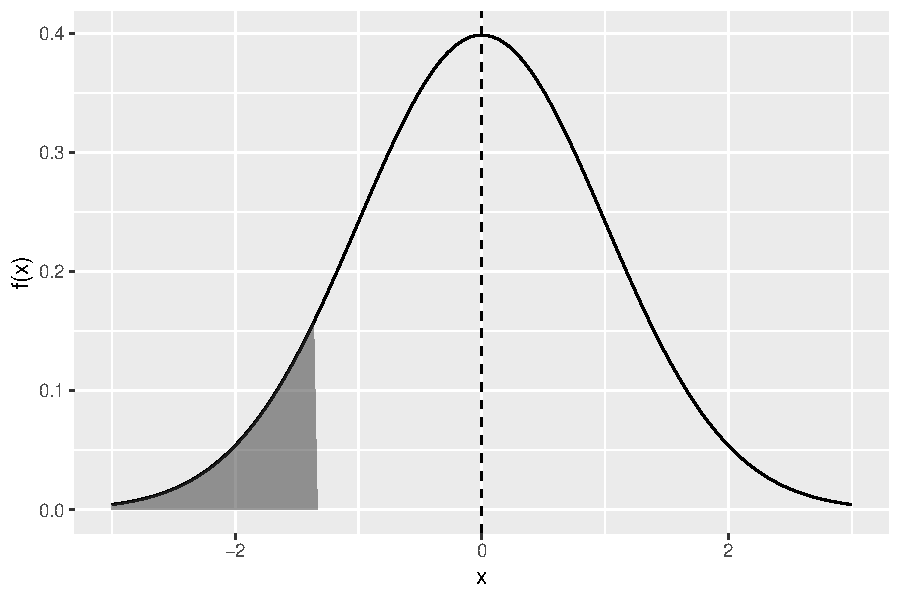
\includegraphics[height = .35\textheight]{figure/exercise-20-6}
    &
    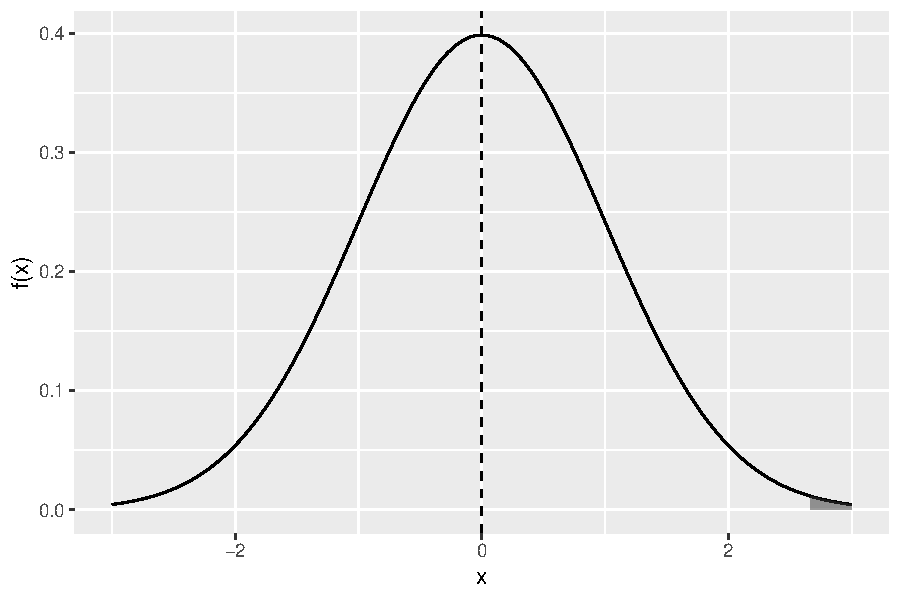
\includegraphics[height = .35\textheight]{figure/exercise-20-7}
    &
    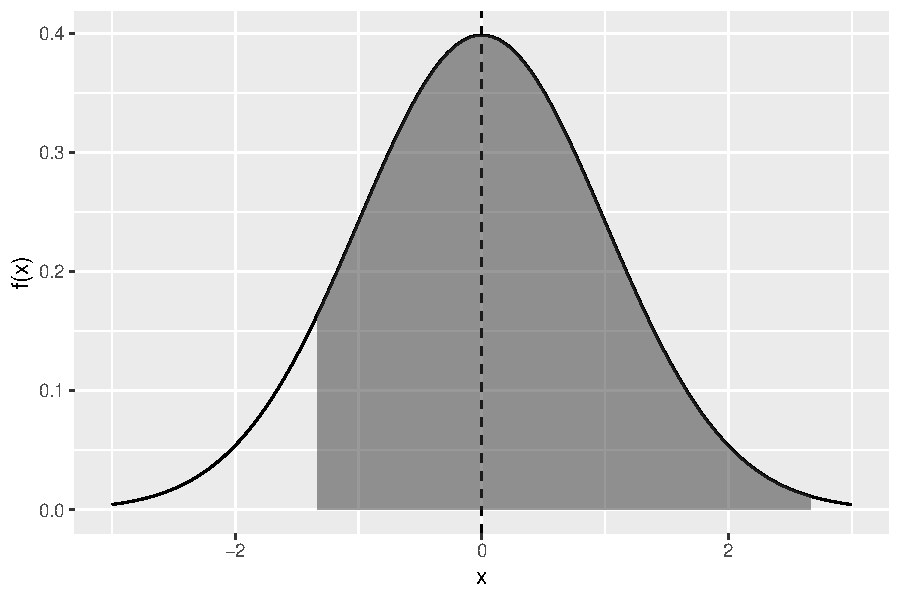
\includegraphics[height = .35\textheight]{figure/exercise-20-8}
    \end{tabular}
    \end{center}
  \end{block}
  
\end{frame}

\begin{frame}
  \begin{block}{The Empirical Rule}
    If $X \sim \mbox{Normal}(\mu,\sigma^2)$ then
    \begin{align*}
      P(\mu-\sigma < X < \mu + \sigma) & \approx .68\\
      P(\mu-2\sigma < X < \mu + 2\sigma) & \approx .95\\
      P(\mu-3\sigma < X < 3\mu + \sigma) & \approx .997\\
    \end{align*}
  \end{block}
\end{frame}

\begin{frame}
  \begin{block}{\examplectd}
    The adult heights of people assigned to be male and female at birth can be modelled amazingly well by a normal distribution. Suppose that the adult height people assigned to be female at birth is normally distributed with mean 64 inches and standard deviation 3 inches.

    \bigskip
    
    Suppose that the adult height of people assigned to be male at birth is normally distributed with mean 67 inches with standard deviation 3 inches.

    \bigskip

    What is the probability that someone's assigned sex was female if they are over 6 feet tall?
  \end{block}
\end{frame}



\begin{frame}

  \begin{block}{\examplectd}
  \begin{center}
    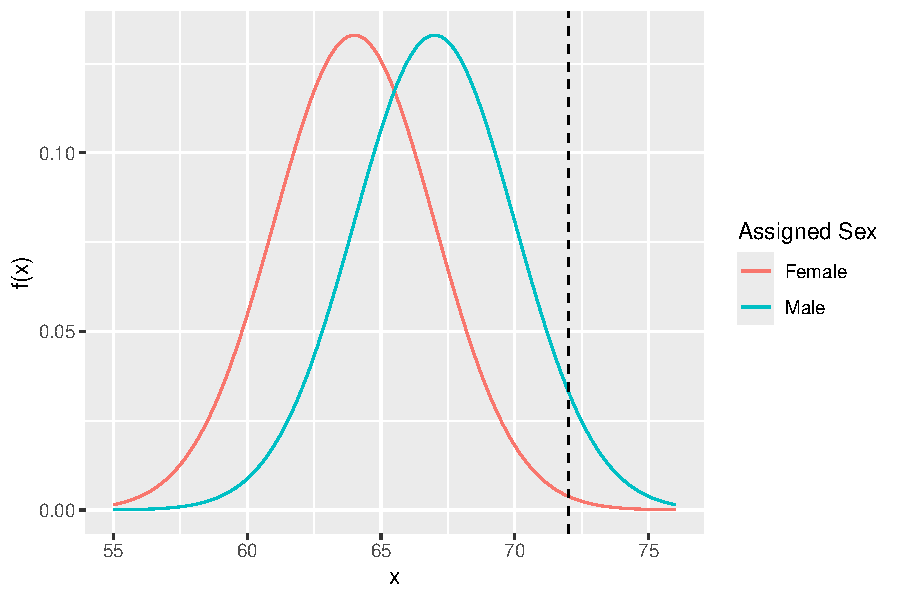
\includegraphics[height = .8\textheight]{figure/exercise-20-1-1}
  \end{center}
  \end{block}
  
\end{frame}

\begin{frame}

  \begin{block}{\example}
     A standard roulette wheel has 37 pockets in which the ball may land. Of these, 18 pockets are red, 18 are black, and 1 is green.

    \bigskip
    
    Suppose that you place \$1 bets that the ball will land in a black pocket on \textbf{200} consecutive games. Let $X$ be the number of times you win.

    \begin{enumerate}[label=\alph*),start=1]
    \item What is the exact probability that you win between 95 and 105 games inclusive?
    \item Approximate this probability with the normal distribution?
    \end{enumerate}
  \end{block}
\end{frame}

\begin{frame}

  \begin{block}{Normal Approximation to the Binomial}
    Suppose that $X \sim \mbox{Binomial}(n,p)$ with $np \geq 10$ and $n(1-p) \geq 10$. Then
    \[
      P(X \leq x) \approx
      P\left(Z \leq \frac{x + .5 - np}{\sqrt{np(1-p)}}\right)
    \]
    where $Z \sim \mbox{Normal}(0,1)$. 
  \end{block}
\end{frame}

\begin{frame}<handout:0>
  \begin{center}
    \Huge{\textbf{Questions?}}
  \end{center}
\end{frame}

\begin{frame}

\begin{block}{\exercise}

\end{block}

\end{frame}

\end{document}
